%%%%%%%%%%%%%%%%%%%%%%% file template.tex %%%%%%%%%%%%%%%%%%%%%%%%%
%
% This is a general template file for the LaTeX package SVJour3
% for Springer journals.          Springer Heidelberg 2010/09/16
%
% Copy it to a new file with a new name and use it as the basis
% for your article. Delete % signs as needed.
%
% This template includes a few options for different layouts and
% content for various journals. Please consult a previous issue of
% your journal as needed.
%
%%%%%%%%%%%%%%%%%%%%%%%%%%%%%%%%%%%%%%%%%%%%%%%%%%%%%%%%%%%%%%%%%%%
%
% First comes an example EPS file -- just ignore it and
% proceed on the \documentclass line
% your LaTeX will extract the file if required
\begin{filecontents*}{example.eps}
%!PS-Adobe-3.0 EPSF-3.0
%%BoundingBox: 19 19 221 221
%%CreationDate: Mon Sep 29 1997
%%Creator: programmed by hand (JK)
%%EndComments
gsave
newpath
  20 20 moveto
  20 220 lineto
  220 220 lineto
  220 20 lineto
closepath
2 setlinewidth
gsave
  .4 setgray fill
grestore
stroke
grestore
\end{filecontents*}
%
\RequirePackage{fix-cm}
%
%\documentclass{svjour3}                     % onecolumn (standard format)
%\documentclass[smallcondensed]{svjour3}     % onecolumn (ditto)
\documentclass[smallextended]{svjour3}       % onecolumn (second format)
%\documentclass[twocolumn]{svjour3}          % twocolumn
%
\smartqed  % flush right qed marks, e.g. at end of proof
%
\usepackage{graphicx}
\usepackage{url}
\usepackage{xcolor}
\usepackage{code}
\usepackage{tabularx}
%
% \usepackage{mathptmx}      % use Times fonts if available on your TeX system
%
% insert here the call for the packages your document requires
%\usepackage{latexsym}
% etc.
%
% please place your own definitions here and don't use \def but
% \newcommand{}{}
%
% Insert the name of "your journal" with
\journalname{International Journal on Software Tools for Technology Transfer}
%
\begin{document}

\title{TSTL: The Template Scripting Testing Language}

%\subtitle{Do you have a subtitle?\\ If so, write it here}

%\titlerunning{Short form of title}        % if too long for running head

\author{Josie Holmes \and
Alex Groce \and
Jervis Pinto \and
Pranjal Mittal \and
Pooria Azimi \and
Kevin Kellar \and
James O'Brien
}

\institute{          Josie Holmes \at
             Department of Geography\\
             Pennsylvania State University\\
           \email{jdh396@psu.edu}
           \and
              Alex Groce, Jervis Pinto, Pranjal Mittal, Pooria Azimi,
              Kevin Kellar \at
              School of Electrical Engineering and Computer Science\\
              Oregon State University\\
              \email{agroce@gmail.com}           %  \\
%             \emph{Present address:} of F. Author  %  if needed
           \and
           James O'Brien \at
          Risk Frontiers\\
           Macquarie University\\
          \email{James.OBrien@mq.edu.au}
}


\date{Received: date / Accepted: date}
% The correct dates will be entered by the editor


\maketitle

\begin{abstract}
The difficulty of writing test harnesses is a major obstacle to the
adoption of automated testing and model checking.  Languages designed
for harness definition are usually tied to a particular tool and
unfamiliar to programmers; moreover, such languages can limit
expressiveness.  Writing a harness directly in the language of the
software under test (SUT) makes it hard to change testing algorithms,
offers no support for the common testing idioms, and tends to
produce repetitive, hard-to-read code.  This makes harness
generation a natural fit for the use of an unusual kind of domain-specific language (DSL). This paper defines a \emph{template
scripting} testing language, TSTL, and shows how it can be used to
produce succinct, readable definitions of state spaces.  The concepts
underlying TSTL are demonstrated in Python but are not tied to it.


\keywords{Software testing \and Domain-specific languages \and
  Explicit-state model checking \and End-user testing \and
  Geographic Information Systems}
% \PACS{PACS code1 \and PACS code2 \and more}
% \subclass{MSC code1 \and MSC code2 \and more}
\end{abstract}

\section{Introduction}

Software test automation encompasses two challenges: (1) automated
execution and determination of results for human-created tests, and
(2) truly automatic generation of tests.  Both are critical for effective,
efficient software testing, but only test generation offers the
potential to discover faults without human determination that a
particular execution scenario has the potential to behave incorrectly.
Automated generation of tests relies on the construction of \emph{test
  harnesses}.  A \emph{test harness} defines the set of valid tests
(and, usually, a set of correctness properties for those tests) for
the Software Under Test (SUT).  This paper presents a language and
tools applying insights from the world of explicit-state model
checking to the problem of producing test harnesses for automated
test generation, whether tests are produced by a exhaustive
state-space exploration as in model checking, or via less
systematic methods.

Building a test harness is a task that even experts in
model checking and automated testing often find painful
\cite{woda08,woda12}.  The difficulty of harness generation is one
reason for the limited adoption of automated testing and model
checking methods by the typical developer who writes unit tests.  This is
unfortunate, as even simple random testing can often uncover subtle
faults.

The ``natural'' way to write a test harness is as code in the language
of the SUT.  This is obviously how most unit
tests are written, as witnessed by the proliferation of tools like
JUnit \cite{JUnit} and its imitators (e.g., PyUnit, HUnit, etc.).  It
is also how many industrial-strength random testing systems are
written \cite{ICSEDiff,AMAI}.  A KLEE ``test harness'' \cite{KLEE} for
symbolic execution is written in C, with a few additional constructs
to indicate which values are symbolic.  This approach is common in
model checking as well: e.g., Java Pathfinder \cite{JPF,JPF2} can
easily be seen as offering a way to define a state space using Java
itself as the modeling language, and CBMC \cite{CBMC,CBMCp} performs a
similar function in C, using SAT/SMT-based bounded model checking
instead of explicit-state execution.  JPF in particular has shown how
writing a harness in the SUT's own language can make it easy to
perform ``apples to apples'' comparisons of various testing/model
checking strategies \cite{JPFRandTest}.


\begin{figure}[b]
{\scriptsize
\begin{code}
op = choice(operations);
val1 = choice(values);
val2 = choice(values);
if (op == op1 \&\& guard1) \{
    call1(val1);
\} else if (op == op2 \&\& guard2) \{
    call2(val1,val2);
\} else if (op == op3 \&\& guard3) \{
    call3(val1,val2);
...
\end{code}
}
\vspace{-0.15in}
\caption {A test harness in the SUT's language.}
\label{fig:badharness}
\end{figure}

Unfortunately, writing test harnesses this way is a highly repetitive
and error-prone programming task, with many conceptual ``code clones''
(e.g. Figure \ref{fig:badharness}). A user faces difficult choices in
constructing such a harness. For example, the example harness always assigns {\tt val2} even
though {\tt call1} only uses {\tt val1}, to avoid having to repeat the
choice code for calls 2 and 3.  The harness is almost certainly
sub-optimal for  random testing, where the lack of any
memory for previously chosen values can make it hard to exercise code
behaviors that rely on providing the same arguments to multiple method
calls (e.g., {\tt insert} and {\tt delete} for container classes).
The construction of a harness becomes even more complex in realistic
cases, where the tested behaviors involve building up complex types as
inputs to method calls, rather than simple integer choices. For
example, consider the problem of testing a complex Python library.  Figure
\ref{fig:MakeFeatureLayer} shows a portion of the Python documentation
for one function in the ArcPy \cite{ArcPy} site
package for Geographic Information Systems (GIS) automation.  Rather than taking a single integer, this
function call requires complex inputs --- a feature class or
layer, an SQL expression, and other complex types that we can assume
are also difficult to construct.  A harness testing a typical
real-world library must manage the creation of values of many such complex types.
Moreover, because building up function inputs is itself complicated
and requires complex method calls, these values cannot simply be produced on each iteration, but must be
stored and selected for use in future calls.
The code quickly becomes hard to read, hard to maintain, and hard to
debug.  In some cases \cite{AMAI} the code for a sophisticated test
harness approaches the SUT in complexity and even size!  The code's
structure also tends to lock in many choices that would ideally be configurable.

\begin{figure}[t]
{\scriptsize
\begin{code}
MakeFeatureLayer\_management(in\_features, out\_layer, {where\_clause}, {workspace}, {field\_info})
   
   Creates a feature layer from an input feature class or layer file. The layer
   that is created by the tool is temporary and will not persist after the session
   ends unless the layer is saved to disk or the map document is saved.
    
INPUTS:
 in\_features (Feature Layer):
   The input feature class or layer from which to make the new layer. Complex
   feature classes, such as annotation and dimensions, are not valid inputs to this tool.
 where\_clause \{SQL Expression\}:
   An SQL expression used to select a subset of features. For more information on
   SQL syntax see the help topic SQL reference for query expressions used in ArcGIS.
...
\end{code}
}
\caption{Documentation for a function in Esri's ArcPy site package.}
\label{fig:MakeFeatureLayer}
\end{figure}

One of the most important of these locked-in choices is the  test generation
method.  Writing a harness by hand usually makes it hard to try out
new strategies.   Writing novel testing strategies in even such
an extensible platform as Java Pathfinder is hardly a task for the
non-expert.
The harness in Figure \ref{fig:badharness} may support random testing and
some form of model checking, if it is written in Java and can use JPF
or a library for adaptation-based testing \cite{ISSRE12}. Such a
harness will likely be completely inflexible as to generation method if written in Python, C,
or another language without that level of tool support.

What the user really wants is to simply provide a concise version of the information in
Figure \ref{fig:MakeFeatureLayer}, some configuration details (e.g., how many
feature classes to keep track of at once), and then try different test
generation methods.  While some automated testing tools for Java \cite{FA11,Pacheco}
can automatically extract
method signatures from source code and produces tests,  
using such a tool locks a user into one test generation method.
Completely automatic extraction also often fails to handle
the subtle details of harness construction, such as defining guards
for some operations, or temporal constraints between API calls that
are not detectable by simple exception behavior.  Understanding
problems with automatic extraction can be hard with large libraries,
since the extraction tends to either produce internal data structures
only or produces a huge, impenetrable mass of code. The user \emph{wants} a
declarative harness, but often \emph{needs} to program critical details of a
harness, and build understanding of the system by performing harness development in
small, incremental steps.

\subsection{Contributions}

In this paper we describe a complete, Domain Specific Language (DSL)-based approach that combines
a simple means to produce a declarative harness with the full power of
a complete programming language.  TSTL (the Template Scripting Testing
Language) compiles a declarative description of system state and
actions into a library in the language of the System Under Test
(SUT).  This library allows the creation of objects providing an API
for testing the SUT, including support for state comparison,
abstraction, backtracking, automatic test case reduction, code coverage, and support
for sophisticated regression testing.

Using an ongoing case study,
we show how to apply TSTL and its tool suite to a large, real-world software
library used in critical applications.  The test effort has been driven and directed not by a
software testing researcher (as is the usual case), but by a domain
expert in the Geographic Information Systems (GIS) SUT.  In the
course of this effort, multiple faults and undocumented restrictions of the library
under test have been discovered, and the TSTL language and tool suite have
been transformed from a research prototype into a complete system for
software testing.

This paper presents the most complete presentation of the TSTL
language and tools, and we hope that it satisfies three critical goals:

\begin{itemize}
\item First, would-be users wanting to take advantage of automated
  test generation should be able to base their own testing
  efforts using TSTL on the example code in this paper (and that available
  in the TSTL github repository \cite{tstl}).
  This paper thus completely describes the concepts behind TSTL, the
  semantics of the language, and the tools available in TSTL.
  Previous papers on TSTL \cite{NFM15,ISSTA15} reported a much less full-featured version of the
  language using a difficult-to-read syntax.

\item Second, researchers should be able to use the information in this paper to
  extend existing TSTL tools or build their own tools to explore novel
  test generation strategies, automated debugging methods, and other
  research prototypes.  TSTL enables easy comparison of
  methods in a framework reducing the burden of implementation
  and avoiding irrelevant differences in performance due to underlying
  infrastructure.  The growing set of SUTs
  included in the TSTL distribution, which includes large and widely
  used Python libraries, can provide benchmarks for
  experimental efforts.  

\item Finally, unlike previous publications on TSTL, this paper
  emphasizes the fact that TSTL, unlike other testing DSLs or tools,
  at heart transforms a definition of valid tests (and properties) for
  a System Under Test into a \emph{programming language interface} for testing
  that system.  Tests in TSTL are not inaccessible entities internal to
  a tool,
  or only represented as unit tests (i.e., programs) that cannot be
  easily manipulated and analyzed, but first-class objects in the
  language of the System Under Test.  To our knowledge, this approach
  to testing has not been previously explored, and it was not
  emphasized (or even clearly presented) in earlier publications on TSTL.
\end{itemize}


The organization of this paper is as follows.  In Section
\ref{sec:dsltest} we present the basic idea of a DSL for testing, and
distinguish TSTL from other testing DSLs.  Section \ref{sec:arcpy} 
provides background on the ArcPy GIS case study used throughout the
paper.  Section \ref{sec:lang} provides a full description, with
examples, of the core TSTL language and semantics.  Section
\ref{sec:tools} describes the tools included with TSTL, and
Section \ref{sec:build} describes how researchers and developers can
build their own TSTL-based testing tools to support additional
testing, debugging, or regression strategies.  Section
\ref{sec:langext} introduces the novel TSTL concept of making testing
a first-class activity in a programming language, similar to how other
libraries make GIS (ArcPy), scientific computing (NumPy \cite{NumPy},
SciPy \cite{SciPy}) or bioinformatics
(QIIME \cite{QIIME}, Biopython \cite{biopython}, scikit-bio \cite{scikitbio}) activities simple to use in either a scripted or
interactive manner.  Faults discovered
using TSTL, in ArcPy and other systems, are described briefly in Section
\ref{sec:bugs}.  We survey the most closely related work in Section
\ref{sec:related}, and summarize our conclusions in Section \ref{sec:conclusion}.

\section{Domain Specific Languages for Testing}
\label{sec:dsltest}

The nature of test harness construction suggests the use of a
\emph{domain-specific language} (DSL) for testing \cite{ISOLA12}.  DSLs
\cite{Fow10} provide abstractions and notations to support a
particular programming domain. The use of DSLs is a formalization of
the long-standing approach of using ``little languages,'' as advocated by Jon Bentley in a
Programming Pearls column \cite{LitLang} and exemplified in such system
designs as UNIX.  DSLs typically come in two forms: \emph{external}
and \emph{internal}.  An external DSL is a stand-alone language, with
its own syntax.  An internal DSL, also known as a domain-specific
embedded language (DSEL), is hosted in a full-featured programming
language, restricting it to the syntax (and semantics) of that
language.  Many attempts to define harnesses can be seen as internal
DSLs \cite{UDITA,ISSRE12,JPF2,CBMCp,KLEE}.  Neither of these choices
is quite right for test harnesses.  Simply adding operations for
nondeterministic choice still leaves most of
the tedious work of harness definition to the user, and makes changing
testing approaches difficult.  With an external DSL, the user
must learn a new language, and the easier it is to learn, the less
likely it is to support the full range of features needed.

A novel approach is taken in recent versions of the SPIN model checker
\cite{SPIN}.  Version 4.0 of SPIN \cite{ModelDriven} exploited the
fact that SPIN works by producing a C program from a PROMELA model
to allow users to include calls to the C language in their PROMELA models.  The
ability to directly call C code makes it much easier to model check
large, complex C programs \cite{AMAI,ModelCode}.  C serves as a
``DSEL'' for SPIN, except that, rather than having a domain-specific
language inside a general-purpose one, here the domain-specific
language hosts a general-purpose language.  A similar embedding is
used in {\tt where} clauses of the LogScope language for testing Mars
Science Laboratory software \cite{scriptstospecs}.  We adopt this
approach for our own language and embed the general-purpose language (for expressiveness) in a
DSL (for concision and ease-of-use).

The most significant difference between TSTL and other DSLs for
testing and verification, including SPIN, is that most such systems
are primarily intended to be used as stand-alone tools.  Whether model
checkers \cite{SPIN,JPF2}, model-based testing tools \cite{Taxonomy},
or random testing tools \cite{Pacheco}, these systems are primarily
designed as ``things to \emph{run on} the system under test.''  TSTL
can operate in this manner, but at heart it transforms a definition of
valid tests into a library for creating, executing, manipulating, and
analyzing test cases.  An experienced TSTL user can interact with TSTL
at an interactive command prompt in the language of the SUT, creating,
saving, and modifying tests on-the-fly.  TSTL tools are simply
scripted formalizations of this mode of use, automating repetitive
tasks.  Such an approach is not possible with any other tool of which we
are aware.  Many tasks that are constrained to the functionality provided
by  tools included in other systems (e.g., replay of regression tests) in
TSTL are simplified and made flexible by this approach.

\subsection{TSTL: The Template Scripting Testing Language}

TSTL is based on understanding a test harness as a declaration
  of the possible actions the SUT can take, where these actions are
defined in the language of the SUT itself, with the full power
of the programming language to define guards, perform
pre-processing, and implement oracles.  Our particular approach is
based on what we call \emph{template scripting}.

The \emph{template} part of the name captures the fact that our method
proceeds by processing a harness definition file to output code that
enables testing, much  as SPIN processes PROMELA/C.  The harness
description file consists of fragments of code in the SUT's language
that are expanded, via the TSTL compiler, into a class that allows
an independently written test generation or manipulation tool to
generate, execute, or replay tests, without knowing
any details of the SUT.
A TSTL harness defines a \emph{template} for action definition, and
the compiler 
instantiates the template exhaustively.  The \emph{scripting} aspect indicates
TSTL is designed to be very lightweight and as easy for
users to pick up as a popular scripting language.  TSTL
works best when the SUT language is very
concise, like most scripting languages, making ``one-liners'' of action
definition possible; our initial implementation \cite{tstl} is therefore for
Python\footnote{We also have released a beta version of TSTL for Java \cite{TSTLJava}, to show
 that testing code in non-scripting languages is also possible.}.

\begin{figure}
{\scriptsize
\begin{code}
@from arcpy import *
\vspace{0.1in}
pools:
  <fc> 3 CONST             \# A feature class contains only lines, points, or polygons
  <newlayer> 3 CONST
  <op> 2 CONST 
  <val> 2 CONST
  <whereclause> 2 CONST    \# SQL clause to limit objects in new layers
  <fieldname> 2 CONST      \# Extracted from the shape files
  <fieldlist> 2
\vspace{0.1in}
actions:
\vspace{0.1in}
<fc> := <["d1.shp", "d2.shp", "d3.shp"]>  \# Just shapefiles for this example
<newlayer> := <["newl1", "newl2", "newl3"]>
\vspace{0.05in}
\{IOError\} <fieldlist> := ListFields(<fc>) \# Extract fields from a feature class
len(<fieldlist,1>) >= 1 -> <fieldname> := <fieldlist> [0].name 
<fieldlist> = <fieldlist> [1:] \# Skip to next field
\vspace{0.05in}
<op> := <[">", "<", "<=", ">=", "=", "!="]>
<val> := <1..10>
<val> = <val> * 10
<val> = <val> + 1

<whereclause> := '"' + <fieldname> + '" ' + <op> + str(<val>)
<whereclause> = <whereclause> + ' AND ' + <whereclause>
<whereclause> = <whereclause> + ' OR ' +  <whereclause>
<whereclause> = 'NOT' + <whereclause>

\{ExecuteError\} MakeFeatureLayer\_management(<fc>,<newlayer>)

\{ExecuteError\} MakeFeatureLayer\_management(<fc>,<newlayer>,where\_clause=<whereclause>)
\end{code}
}
\caption{A small TSTL file to test one ArcPy function.}
\label{fig:makefeaturelayer}
\end{figure}

\begin{figure}
{\scriptsize
\begin{code}
import sut, random, time
rgen = random.Random()
sut = sut.sut()
NUM\_TESTS = 1000
TEST\_LENGTH = 200 
for t in xrange(0,NUM\_TESTS):
   sut.restart()
   for s in xrange(0,TEST\_LENGTH): 
       action = sut.randomEnabled(rgen)
       r = sut.safely(action)
       if len(sut.newBranches()) > 0:
          print time.time(),'NEW BRANCHES:', sut.newBranches()
       if (not r) or (not sut.check()):
          pred = sut.failsCheck if r else sut.fails
          print 'TEST FAILED:', sut.error() 
          R = sut.reduce(sut.test(), pred)
          N = sut.normalize(R, pred) 
          sut.generalize(N,pred)
\end{code}
}
\caption{A simple random tester using the interface provided by TSTL.}
\label{fig:rt}
\end{figure}

Figure \ref{fig:makefeaturelayer} shows a simple TSTL harness for the
function documented in Figure \ref{fig:MakeFeatureLayer}.  Even this
short harness supports constructing SQL where clauses of arbitrary
length and selecting field names based on data files.  Figure
\ref{fig:rt} shows a simple pure random test generator that can test
any SUT (including this one) with a TSTL-defined harness.  This
harness, in 20 lines of code, not only provides automated test
generation, but continuous reporting of incremental branch coverage,
delta-debugging \cite{DD} for reduction of failing tests, and
additional TSTL-specific post-processing that further reduces the size
and complexity of test cases for debugging.  The brevity of the test
generator, no matter how complex the SUT, is made possible by the
common functionality of all TSTL-generated testing interfaces.  The
TSTL compiler produces a Python (or other target language) class that allows a test generation or manipulation
tool to view a testing problem as exploration of a (possibly infinite)
graph of states.  Transitions in the graph are the available test actions, executed in the underlying language, and are guarded by both TSTL
restrictions on the semantics of valid tests and user-defined guards
on system behavior.  States include both the (possibly unknown) state
of the SUT and the TSTL state, including pools of values to be used in actions.

In this simple example, the only ``oracle'' is the implicit property
that the system should neither crash nor raise an unexpected
exception.  For testing many systems, this is sufficient: we have
discovered real bugs in many Python libraries with only this level of
checking, similar to most of what a tool such as Randoop
\cite{Pacheco} or JCrasher \cite{CsallnerS04} checks.  TSTL also
checks arbitrary assertions/invariants defined in the language of the
SUT, supporting traditional property-based testing
\cite{ClaessenH00,hypothesis} (described in Section \ref{sec:property}).  Finally, TSTL includes sophisticated
support for differential testing \cite{Differential,ICSEDiff}, where a
system is tested with respect to the behavior of a reference library.
TSTL makes it easy to wrap a reference system to account for expected
differences, and supports partial reference testing (see Section \ref{sec:differential}).

\section{Motivating Case Study: Esri ArcPy}
\label{sec:arcpy}

Esri is the single largest GIS software vendor, with about 40\% of
global market share.  Esri's ArcGIS tools are extremely widely used
for GIS analysis, in government, scientific research, commercial
enterprises, and education.  Automation of complex GIS analysis and
data management is essential, and Esri has long provided tools for
programming their GIS software tools.  The newest such method,
introduced in ArcGIS 10.0, is a Python site-package, ArcPy
\cite{ArcPy}.  ArcPy is a complex library, with dozens of classes and
hundreds of functions distributed over a variety of of toolboxes.
Most of the code executed in carrying out ArcPy functions is the code
for the ArcGIS engine itself.  This source code, written in C++
(amounting to millions of lines), is
not available.  The source code for the latest version (10.3) of the
Python site-package alone, however, which interfaces with the ArcGIS
engine, is over 50,000 lines of code.  This is a very large system
(especially given the compactness of Python code), comparable in size
to the largest software systems previously tested using automated test
generation, such as core Java and Apache libraries
\cite{FA11,Pacheco}.

In order to improve the reliability of ArcPy, we are developing a
framework for automated testing of ArcPy itself, as well as libraries
based on ArcPy.  The TSTL harness for ArcPy is already more than six times as
large as the next-largest such definition previously implemented in
TSTL, even though the harness so far only includes a small portion of ArcPy
API (Application Program Interface) calls. The first stage of testing has resulted in discovery of
multiple faults in ArcPy/ArcGIS, and has required modifications to the
TSTL language and, especially, to the tool chain supporting test replay,
debugging, and test case understanding.

%One of the contributions of this paper is a more in-depth discussion
%of the problems, challenges, and tool utility aspects of testing
%software than is typical in most research papers in the field.  Such
%papers are (understandably) typically focused on novel algorithms or
%empirical evaluations of known methods, rather than the practical aspects of finding
%and understanding faults in a real-world software system.


%\subsection{Automated Testing for the Rest of the World}

Previous work on automated test generation for APIs has been largely carried
out by software testing researchers only, or (at most) by software
testing researchers working with individuals who are primarily
software developers.  This paper describes TSTL in the context of a
testing effort largely directed (and coded) by the first author, who is not a
software developer by profession or education, but a GIS analyst.
The problem of end-user testing
\cite{burnettEUSE,Silos,rothermelTOSEM} is long-standing.  Previous
work in the field has often focused on
non-traditional programming: e.g. spreadsheets
\cite{rothermelTOSEM}, visual languages, or machine-learning systems
\cite{OnlyOracle}.  TSTL is partly designed to allow a user who is
familiar with a software library but not expert in software testing
techniques to test a traditional software API library.  In one sense,
this is a less difficult scenario than spreadsheets
or visual forms, in that the testing is directed by an individual used
to writing and thinking about code.  The concepts in
automated software testing are most easily understood by those
who are also familiar with a conventional
programming language.  On the other hand, ArcPy is
not a small user-developed program but a large, complex system.
ArcPy was also not written by the end-user, or by any of the authors
of this paper, nor have the authors received any assistance in the
effort from Esri.

Automated testing systems more advanced than a simple hand-written
loop generating a few random inputs to a handful of functions, or more
complicated to use than a fully push-button system are often
considered too difficult for practical use even by software developers
or software QA staff \cite{ISSRE12}. Even ``push-button'' tools for
automated testing are sometimes difficult for expert users to install,
apply, and configure \cite{AMAI,CFV08,ISSRE12}.  TSTL aims to be
relatively easy to use for anyone familiar with basic Python
development.  By avoiding the use of a toy problem and presenting TSTL
in the context of a more typical real-world system (vs. e.g., a simple
container class), we hope to make it easier to apply to other
real-world systems.
%One goal of this work
%has been to mature the TSTL language and tool chain so Python
%programmers from all backgrounds can easily apply it to their
%automated testing problems, with tools approximately as easy to use as
%other Python developer tools.

%The second major contribution of this paper is therefore a presentation of an
%approach to automated testing that has been chosen by a GIS analyst, not a
%software developer or testing researcher.  Moreover, we present this
%paper as a proof-of-concept that modern automated testing, even in a
%highly interactive, non-push-button form, can be used by a motivated
%domain expert, with the support of  a domain-specific language
%\cite{Fow10} and a set of tools for generating, analyzing, and replaying tests.




\section{The TSTL Harness Language}
\label{sec:lang}

The TSTL compiler takes as input a harness template file, and produces
as output a Python class file that implements an interface other tools
(or even users working interactively)
can use to perform testing on the SUT via an SUT-independent interface.

The harness in Figure \ref{fig:MakeFeatureLayer} shows many of the
basic features of TSTL.  The basic structure of a TSTL harness
consists of three parts, usually written in order.  First, harness
code prefixed by an {\tt @} or enclosed in {\tt <@ @>} is treated as
raw Python code, and essentially not interpreted by the TSTL
compiler.  This code is reproduced almost literally in the output
file\footnote{TSTL does have to scan {\tt import}s to re-load modules, and also pre-processes function
  definitions to support
pre- and post-conditions.}.  Second, there is a preamble that almost
always defines a set of \emph{value pools} for use in testing, but
also may include information on logging, correctness properties,
source code locations for code coverage analysis, and other basic
information that applies to the entire harness.  Finally, the bulk of
a TSTL harness (and the only non-optional element) is a set of
\emph{action definitions}.  Actions are the possible steps to be taken in
testing, and define the set of possible tests.

The original version of TSTL \cite{NFM15} required cumbersome use of Python
functions to implement many simple operations, including guards.  Current TSTL extends
the language to make it possible to define very complex test spaces
using only pools and actions, with helper functions only required for
the usual reasons of abstraction and readability.

\subsection{The Essentials of Pools and Actions}

In TSTL, tests usually consist of assignments to value pools and
function calls making use of those values.  These are the most common
forms of actions.  Value pools are meta-variables in the target
language, and support the complete set of types of the underlying
language.  A pool can contain simple types such as integers, or more
complex types such as functions, container classes, file handlers, or
even TSTL testing objects (to support testing TSTL itself).  The
notion of an action in TSTL is similarly completely general:
\emph{any fragment of code in the host language can be an action}.
Usually, it is most convenient to encapsulate complex actions by
defining functions that perform the desired behavior, and making the
action a call to such a function, but this is not required.  As
Andrews et al. have shown \cite{AndrewsTR}, this pool-and-action approach is
sufficient to express the full generality of unit tests, in any
language\footnote{In fact, TSTL tests are somewhat more general than
  this already very general and expressive form, in that we do not
  disallow loops and conditions in actions.}.

In order to make the core ideas clear,
consider part of the harness shown in Figure \ref{fig:MakeFeatureLayer}, defining how to
generate values used in SQL where clauses.  The following, by itself,
is a valid TSTL harness (albeit one that cannot discover any
faults, since it performs no actions beyond simple integer addition):

{\scriptsize
\begin{code}
pools:
  <val> 2 CONST
\vspace{0.05in}
actions:
\vspace{0.05in}
<val> := <1..10>
<val> = <val> + 1
\end{code}
}

There is only one pool, named {\tt val} (optionally labeled as {\tt CONST} to
indicate that its value does not change unless it appears on the left
hand side of an assignment).  The pool has room to store
two values.  The state of the SUT is defined by the state of all
pools.  Initially, all pools are set to a special value ({\tt None}) indicating the
pool has not been initialized.  For the most part, we can think of the
{\tt val} pool as two Python variables {\tt val0} and {\tt val1}.  Another
way to think about a pool is as a kind of informal ``named type,''
with a limited set of variables that can contain the ``type'' and all
possible action sequences that assign to its pool values serving as
its specification.  In Python it is not necessary to specify the
actual type
of a value pool, though an optional {\tt : type} notation enables TSTL
to perform runtime type-checking and ensure pools never contain
incorrect types.

In this simple example, the only actions are initialization of a {\tt
  val} and incrementing a {\tt val}.  Again, we emphasize that an
action can in general be an arbitrary Python statement.  Actions that
include the {\tt :=} form of assignment (a TSTL, not Python,
operation) initialize pool values.  When {\tt <val>} appears in an
action, that represents all possible pool values with that name: for
our simple example, either {\tt val0} or {\tt val1}.  An integer range
is represented by {\tt <i..j>}, and TSTL expands such ranges to
produce an action with each possible choice. The first line in the
actions section of this harness translates to 20 different possible
actions:

\begin{figure}
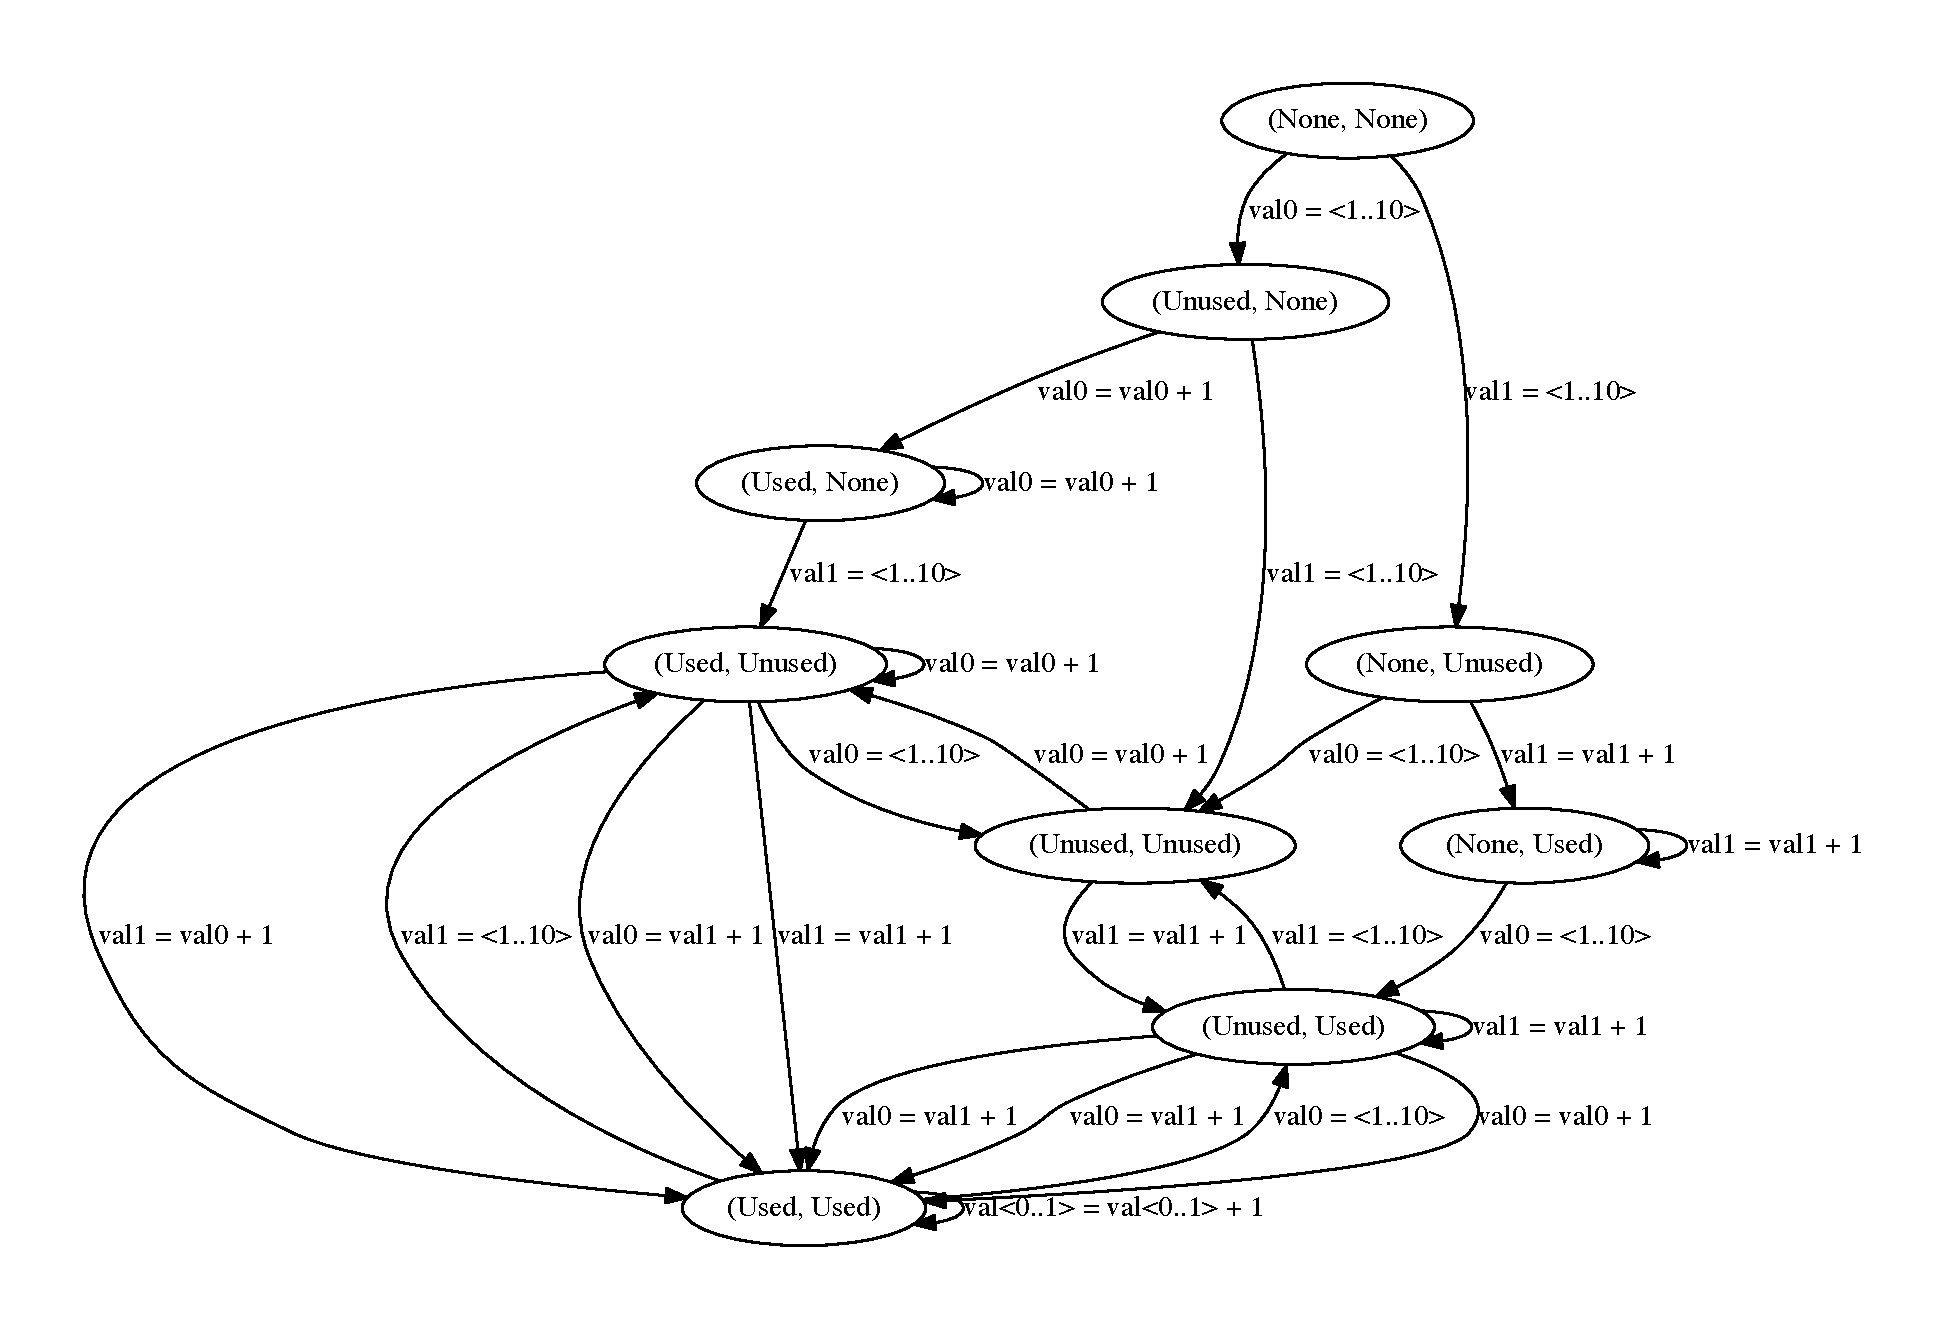
\includegraphics[width=\columnwidth]{states}
\caption{Constraints on actions in a test, based on pool states}
\label{fig:poolacts}
\end{figure}

{\scriptsize
\begin{code}
val0 = 1
val0 = 2 ...
val0 = 10
val1 = 1 ...
val1 = 10
\end{code}
}

From the initial state of the system, only these 20 actions are
\emph{enabled}.  \emph{Enabled} actions are those that can be executed in the
current state; the complete set of actions defined by a TSTL harness is always
finite, and the enabled set is always a subset of that finite set.  The first concept that is essential to understanding
TSTL semantics is that at any state of the
system, the only actions that are enabled are those that do not
\emph{use} any non-initialized pool values.  Any appearance of a pool
value is considered a \emph{use}, with the single exception of the left-hand-side of a
{\tt :=} initialization (not normal assignment)\footnote{The definition of
use is the only distinction between {\tt :=} and normal Python
assignment; {\tt :=} is implemented as Python assignment, and appears
as such when test cases are printed.}.  The second concept is that a
value that has been initialized
cannot be initialized (appear on the lhs of {\tt :=}) until after at
least one action
that uses it has been executed.  Figure \ref{fig:poolacts} shows the
consequences of these rules for the simple value assignment harness
above.  The nodes in the graph are labeled with {(\tt state(val0),
  state(val1))}, where state is
either {\tt None} (uninitialized), {\tt Unused} (initialized
but never used) or {\tt Used} (initialized and used at least once).
Starting from the initial state {\tt (None, None)}, a valid test is any path
through the graph. 

Tests that can be produced by this harness include, therefore,
sequences like  {\tt val0 = 3; val0 = val0 + 1; val1 = 4; val1 = val0
  + 2} and {\tt val1 = 10; val0 = 6; val0 = val1 + 1; val0 = 2; val1 =
  15}.  However, {\tt val0 = val0 + 1; val0 = 2} and
{\tt val0 = 1; val1 = 1; val1 = 4} are not valid tests, because they
either use an uninitialized pool value, or re-initialize an unused
pool (a clearly useless action sequence).

\subsection{Guards, Post-Conditions, and Properties}
\label{sec:property}

The example TSTL harness in Figure \ref{fig:MakeFeatureLayer} shows a
few other important core elements of TSTL.  First, choice templates
are not limited to integer ranges, but can include arbitrary items in
a list, e.g, {\tt <fc> := <["d1.shp", "d2.shp", "d3.shp"]>}.  Note
that while in the example these items are (string) constants, they can
be arbitrary expressions to be computed at runtime, or even incomplete
code fragments that are only valid when combined with the rest of the action.
Second, when an action raises an uncaught exception, this is normally
considered a test failure.  Prefixing an action with a set of
exception names in curly braces (e.g., {\tt \{IOError\}}) indicates
that some exceptions are expected, and do not indicate a failure.

More critically, actions can also be prefixed by arbitrary guards, using
the syntax {\tt guard -> action}.  The simple ArcPy harness chooses
field names for SQL by first extracting a list of all fields in some
feature class.  It then allows a field name to be chosen by taking the
name of the first field in the list.  However, since the harness also
allows the list of fields to be stepped through by discarding the
initial element, the name extraction has to be guarded to ensure that
tests won't try to extract names from an empty field list:  {\tt
  len(<fieldlist,1>) >= 1 -> <fieldname> := <fieldlist> [0].name}.
The {\tt <fieldlist,1>} construct, which can also be used outside of a
guard, indicates that this pool value should not be produced using
normal template expansion (instantiated as both {\tt fieldname0} and
{\tt fieldname1}) but rather that it should copy (textually, not a
copy of the object but the same variable use) the comma indexed
appearance of that pool in each expansion (indexing starts from 1).  This makes sure the guard
is over the same pool value that is used in the action.

TSTL also supports post-conditions on actions, in the form {\tt action
  => post-condition}, where the post-condition is checked after the
action is performed.  For example, because some known ArcPy bugs
involve addition of incorrect characters to field names in a database,
we could add code to check that field names in feature classes never
change from their initial values.  We can make sure that a library
call to add a field to a feature class adds it to a database of all
field names collected at the start of testing, and collect the set of
fields in each feature class file at the beginning of each test,
storing these in a dictionary.  This example code shows two more
features of TSTL: TSTL supports {\tt init:} code in the preamble,
which is called before each test starts.  Ending a line in a backslash
indicates the action continues on the next line of the file.

{\scriptsize
\begin{code}
init: <fieldnames> = getAllFieldNames(getFeatureClasses())

\{ExecuteError\} not (<fc,1> in <hascursor>) -> \\
   AddField\_management(<fc>,<fieldname>,<fieldtype>); \\
   <fieldnames> [<fc,1>].add([<fieldname,1>])

\{IOError\} <fieldlist> := ListFields(<fc>) \\
  => sorted(<fieldlist,1>) == sorted(list(<fieldnames> [<fc,1>]))
\end{code}
}

Note the additional guard on adding fields --- we have discovered that
adding a field to a feature class that has any database cursors active
tends to crash ArcPy.  For more complicated post-conditions, the construct {\tt
  pre<(expr)>} allows access to values of expressions from before the
action was executed, as a further convenience for expressing properties.

When an assertion is an invariant on all post-action states, it can be
included in the preamble.  To check field names we would write {\tt
  property: sorted(ListFields(<fc>))==sorted(list(<fieldnames>
  [<fc,1>]}.

This property checks all feature classes, not just those whose
fields are extracted.  The advantage is that the property will
catch problems even if we never construct a {\tt fieldlist}; the
disadvantage is that testing slows to check all field names for all
feature classes, after every action.

\subsection{Differential Testing Support}
\label{sec:differential}

Another useful feature of TSTL is the ability to create
\emph{reference} pools, where every action on pool values is mirrored
by an action on a reference version of that pool.  This makes it
possible to perform differential testing \cite{Differential} on a
per-pool basis, rather than at the whole-system level, allowing
complex partial specifications.  The idea is that the behavior of some
pool (which could be the entire SUT state, in the extreme) can be
compared to a reference implementation that provides the same
observable behavior.  The classic example is the idea of testing a C
compiler by checking that the output of running a deterministic, well-defined
C program compiled under two different compilers (or optimization
levels) is the same.  If the systems differ, one must be incorrect.  A
simpler example is checking a set-like data structure against a
well-tested reference implementation.  The TSTL distribution includes
an example where an AVL tree implementation is checked against the
Python set implementation.

Differential testing can also be useful for applications other than
testing complete systems against each other; the SUT may provide
different implementations of essentially the same functionality,
serving as a reference for itself (compilers are often tested against
their own code, with optimization turned off). In ArcPy we may want to
ensure that operations are deterministic: no GIS operations produce
different results, given the same underlying starting feature class
data.  Assuming in raw Python in the preamble we have defined {\tt
  identityFunction} as an identity function and {\tt copyFCName} as a
function that takes a feature class name and transforms it into a
generated name for a reference copy of the feature class, the
following mirrors all actions on feature classes on a reference copy,
and checks that the feature class and its reference always have the
same fields.

{\scriptsize
\begin{code}
pools:
  <basefc> 2 CONST
  <fc> 2 CONST REF

<basefc> := <[``d1.shp'', ``d2.shp'', ``d3.shp'']>; \\
  CopyFeatures\_management(<basefc,1>,copyFCName(<basefc,1>)
<fc> := identityFunction(<basefc>)
\{IOError\} <fieldlist> := ListFields(<fc>)

references:
  identityFunction ==> copyFCName

compares:
  ListFields
\end{code}
}

When instantiating the action templates, TSTL always produces a copy
of every action containing any reference pool values.  First, the pools
are replaced with their reference copies; second, all the
syntactic transformations (which can include arbitrary Python regular
expressions) in the {\tt references} declaration are applied, to
produce the appropriate Python expression to evaluate to perform the
action using the reference implementation.
Finally, if any string matches a regular expression in a {\tt
  compares} declaration, the return values or assigned values in the
action are compared with those for the reference version, and a fault
is raised if the results are not equivalent.  In the
ArcPy case, if our {\tt copyFCName} is correctly defined, we can even
check that behavior is equivalent for different underlying data file
formats for feature classes, by treating, e.g., shapefiles as a
reference for a personal geodatabase.  In addition to such simple (and
modular) reference checking, TSTL allows properties to use the value
of a reference pool, with syntax like:

{\scriptsize
\begin{code}
property:  str(<expr>) == str(REF:<expr,1>)
\end{code}
}

\subsection{How to Build a TSTL Harness}

In the introduction, we noted that one problem with automatic
extraction of harnesses by testing tools is that in order to effectively test
complex systems, it is important to incrementally build testing
capability.  Often, as with software development, understanding the
effort as it slowly increases in scope is essential.  TSTL
naturally supports this methodology.  The ArcPy harness, though
complex, was developed by starting with a small number of ArcPy
functions, and determining their parameters.  These functions were
chosen because they were involved in unusual or problematic behavior
experienced by the authors of the paper.  Once
functions have been chosen, and their parameters are known,
developing a harness can often be a clean, iterative process:

\begin{enumerate}
\item Choose a new function (or set of related functions) to include
  in the harness.
\item Determine all parameter types for these functions.
\item If there is no pool that can produce these types, determine how
  to produce these types, and add pools and pool initialization actions for
  those pools.  This may require adding some additional
  functions (in which case, go to step 1 and start with those
  functions, recursively).
\item Add an action to call the function(s) being added.  If relevant,
  allow any expected exceptions, guards, and post-conditions to check.
\item Run testing, examine code coverage and failures to evaluate the
  added harness features, and repeat from step 1.
\end{enumerate}

These steps, combined with occasional refactoring or generalization of
parts of the harness, can effectively test even a large library, while
maintaining tester understanding and control.   In the ArcPy test
harness development, most of the effort was spent in this cycle, with
major exceptions being the implementation of a method allowing users
to provide their own GIS data as a basis for testing, and efforts to
improve the TSTL tool infrastructure to support testing a complex
application in a Windows environment.

%\subsection{Defining Complex Properties}

Note that because TSTL defines the structure of a potentially infinite
number of tests, users are expected to define correctness of a system
via \emph{property-based testing} \cite{ClaessenH00}.  As in
model checking, the correctness of the system is not specified via users
determining the specific output for each test sequence, but by
defining general properties over all executions.  TSTL includes
idiomatic support for common forms of property-based specification,
including invariants, post-conditions on actions, and comparison with
the outputs of a reference implementation \cite{Differential}.

\subsection{TSTL and Other Languages}

At heart, the TSTL ``language'' consists of the syntax and semantics for pools,
nondeterministic choice\footnote{Nondeterministic choice \cite{EWD:Discipline,McCarthy,Floyd,woda12} is both
  inherent in the notion of a TSTL action, and represented more
  concretely by the
  syntactic sugar of the {\tt <[...]>} notations.  Arguably, building
  the language and semantics around nondeterministic choice to
  represent a transition system/state space is the core idea of TSTL.},
guards, pre-conditions, pre- values, and a few other elements on top of
an existing language:  the abstract basis of TSTL has a conceptually
small footprint.

While the implementation effort to compile to an SUT interface in a
different language is considerable, there is no difficulty (beyond
engineering effort) in mapping TSTL to languages other than Python.
In one summer, an advanced high school student was able to produce a
working version for Java \cite{TSTLJava}.  Implementing TSTL for
Scala, Ruby, or even C/C++ would require effort but no research
breakthroughs.  As with the Python and Java TSTL implementations,
there is no need (due to the intentional template structure) to even
parse the underlying language.  The primary development effort is
translating the TSTL ``runtime'' of utility functions to a new
language.  For Scala, Ruby, or Swift we believe this would be quite
trivial.  For C/C++ the relative lack of functional language features
would be frustrating, but certainly not a blocking difficult.
The ideas behind TSTL are abstract and generally
applicable, even if the current implementation is built for Python.



\section{TSTL Tools}
\label{sec:tools}

The following tools are provided in the TSTL distribution on github \cite{tstl}.  Installing the TSTL module allows the compiler, called {\tt tstl}, to be used at the command line.  Other tools are included in the {\tt generators} and {\tt utilities} directories of the distribution as Python scripts.

\subsection{The TSTL Compiler}

Given a harness file defined in the language discussed above, the TSTL compiler generates a stand-alone Python class that allows testing of the SUT.  This generated code does not depend on the TSTL system being installed, only on any modules the testing itself uses, and on whether code coverage is requested.  By default, the compiler produces a class supporting code coverage using the {\tt coverage.py} module, and assumes this is installed.  The TSTL compiler also allows a user to control some fine-grained coverage measures (e.g, is coverage measured during initialization and module reloads?), and force a system to use replay-based backtracking by default.

\subsection{Test Generators}

TSTL comes with a complex, highly configurable, pure random tester (supporting numerous command-line options).  The included random tester provides a number of useful options, of which a subset are shown in Figure \ref{tab:rt}.   

\begin{figure}
{\scriptsize
\begin{itemize}
\item {\tt depth <int>}: Determines the length of generated tests.
\item {\tt timeout <int>}: Determines the maximum time spent generating tests, in seconds.
\item {\tt seed <int>}: Determines the random seed for testing.
\item {\tt maxTests <int>}: Determines the maximum number of tests to be generated.
\item {\tt running}: Produce on-the-fly, time-stamped code coverage information, for analyzing performance of testing algorithms. 
\item {\tt replayable}: Produce a log of the current test, so even it crashes Python the test can be reproduced, delta-debugged, made stand-alone, or otherwise analyzed.
\item {\tt total}: Produce a total log of all test activity, including across resets, for systems where reset is not complete (so tests across resets can be delta-debugged).
\item {\tt quickTests}:  Produce ``quick test'' files \cite{icst14}, each containing a minimal test to cover a set of branches of the SUT. 
\item {\tt normalize}: Apply additional, custom term-rewriting based simplifications of test cases that often further minimize delta-debugged test cases. 
\item {\tt generalize}: Apply generalization that elaborates each failing test with annotations showing similar tests that also fail. 
\item {\tt swarm:}  Apply swarm testing \cite{ISSTA12} to test generation.
\end{itemize}
}
\caption{Some options for the TSTL random test generator.}
\label{tab:rt}
\end{figure}

To our knowledge, TSTL's random tester is the first general-purpose random testing tool to incorporate the powerful swarm testing \cite{ISSTA12} algorithm, which has previously been used to test compilers \cite{ISSTA13,ZhendongPLDI14} and file systems.  TSTL's version of swarm testing is more sophisticated than previously published versions, in that it analyzes the dependency graph of TSTL actions to avoid producing degenerate test configurations, improving performance over naive swarm testing.  In addition to these stable, commonly used options, the random tester includes novel experimental options, such as the ability to guide random testing by a user supplied Markov model or operational profile \cite{Hamlet94}.  TSTL makes implementing novel test generation methods simple, as discussed below.

The base TSTL tools also use the TSTL interface to support explicit-state model-checking \cite{ModelChecking,SPIN}, using either Depth-First-Search (DFS) or Breadth-First-Search (BFS) strategies.  TSTL uses Python's {\tt deepcopy} tools to provide a simple, easy to use interface for automatically storing and restoring pool states, making these algorithms trivial to implement.  There is no fundamental technical difference between performing (theoretically exhaustive) systematic searches of a well-defined transition system or random exploration.  Using the same transition system definition for both purposes has considerable advantages, as pointed out in previous work \cite{woda08}, especially for effectively infinite-state systems where random walks will never saturate and exhaustive searches will never complete.
TSTL can (unlike SPIN or most explicit-state model checkers) apply BFS or DFS search even to systems without support for backtracking.  TSTL's abstract interface to an SUT (transition system) can be configured to provide replay-based simulation of state storage and retrieval.  This is required when, for example, a library uses a C extension and so Python's {\tt deepcopy} does not allow full copying of the state of pool objects, or when the system has hidden global state that cannot be captured in a pool value.  While state storage and backtracking is usually faster than replay, we find that for some systems the opposite is true, particularly for shallow search depths (which are typical for BFS of a complex system).

TSTL also supports custom abstraction of pools.  If a pool is declared with an {\tt ABSTRACT} annotation, the function after the {\tt ABSTRACT} keyword is used to abstract all values for state-matching purposes during exhaustive exploration methods, via the {\tt abstract} function.  The {\tt state} method returns the concrete state of the system (since these are required for backtracking), but applying the {\tt abstract} function to this state returns an abstract version of the state to be used in state matching.  The core of a BFS, for example, can be expressed quite simply, irrespective of whether the system is using state storage and backtracking or replay (or has an abstraction or not) as:

{\scriptsize 
\begin{code}
old = sut.state()
for act in sut.enabled():
   sut.safely(act)
   new = sut.state()
   \# repr produces a hashable string representation
   absNew = repr(sut.abstract(new))
   if absNew not in visited:
      queue.append(new)
      visited[absNew] = True
      ...
   sut.backtrack(old)
\end{code}
}

This loop iterates through all enabled actions from the current state, and adds any not previously visited to the search queue.  Similar code works as the core of a DFS.  Implementing heuristic model checking searches is also trivial, whether those searches are SUT/error specific \cite{EdelkampHeur} or structural \cite{groce-structural}.

While not required for any of our testing efforts thus far, encoding temporal logic checking is also simple.  A B\"uchi automata can be encoded in Python, querying the SUT state and action choices to determine transitions.  Composing this with the SUT state is trivial.  We managed to implement the well-known nested DFS algorithm \cite{DoubleDFS} in less than 40 lines of code, taking the property automata as a tuple input {\tt(initial, trans, accept)}, where {\tt trans: (state, action, sut state) -> state}.

\subsection{Utilities for Test Case Manipulation}

TSTL provides the tools {\tt sandboxreducer} and {\tt standalone} for manipulating saved test cases produced by the random tester or the simple model checkers.  These were developed as part of the ArcPy testing process.  ArcPy faults tend to crash the system (this is also the reason the {\tt total} option was introduced), and thus cannot be simplified for debugging inside the test generator.   The sandbox reducer takes a testing log and, using subprocesses to handle crashes, produces delta-debugged and normalized test cases. It is also useful to report failing tests not as TSTL's internal test file format, but as standalone Python programs that cause a failure.  The {\tt standalone} utility takes a test log or a saved test case and produces a complete, stand-alone Python program that requires neither the generated TSTL interface nor any other TSTL tools.

\begin{figure}
{\scriptsize
\begin{code}
import sut
import glob

sut = sut.sut()

failed = 0
total = 0

for testFile in glob('regressions\\*.test'):
   t = sut.loadTest(testFile)
   total += 1
   if sut.failsAny(t):
       failed += 1
       print testFile,'FAILED:',sut.failure()

print total,'TESTS EXECUTED'
print failed,'TESTS FAILED'

print len(sut.allBranches()),'BRANCHES COVERED'
print len(sut.allStatements()),'STATEMENTS COVERED'
print sut.report('coverage.txt'),'\% STATEMENTS COVERED'
\end{code}
}
\caption{A small script to run stored regression tests}
\label{fig:regress}
\end{figure}


However, use of these tools is often not required.  Figure \ref{fig:regress} shows a simple, but complete, Python script for running regression tests generated using TSTL for a system.  This script examines the {\tt regressions} directory, replays each test in the directory, and reports on failing tests and code coverage.  Such a script can easily be customized to provide different tests for different budgets (e.g., prioritized by time, coverage, or to execute coverage-based 'quick tests').

\subsubsection{ArcPy Regression Generation}

One difficulty for ArcPy users is ensuring that their existing scripts
and tools work on new versions of ArcGIS.  Each recent major release
(10.2 and 10.3) after ArcPy's introduction has potentially included some changes
in the behavior of API calls.  Detecting when such changes cause a
script to break is difficult.  A first step would be an automatic way
to find when the return values for calls differ between ArcPy
versions.
Because installing multiple versions of ArcGIS on the same system is
difficult or impossible, our method for finding differences relies on
choosing a reference version (10.3 in our current efforts), and
generating a set of standalone tests that 1) cover a large amount of
ArcPy functionality, including invalid inputs to functions and 2)
record the return values and exceptions raised by calls.  These tests
can be run on any ArcPy version, and will report differences between
the tests and version 10.3.  Performing this kind of differential
testing \cite{Differential} on old or new major releases, or across 64
bit and 32 bit versions, is easy.  In the long run, we also want to
enable TSTL to produce Python 3.0+ code, for use with ArcGIS Pro,
which uses Python 3.4 instead of 2.7.  This has motivated a branch to
TSTL to support Python 3.0 (unfortunately, Python 3.0 is not fully
backwards compatible with earlier versions, and Python 2.7 is still
the most widely used Python, and non-pro versions of ArcPy only work
with 2.7).

We generate coverage-based regression tests using an approach called \emph{quick
  testing} \cite{icst14,stvrcausereduce}, which takes a set of tests
produced by random testing or model checking, and applies a test case reduction
algorithm \cite{DD} to produce smaller tests that have the same code
coverage as the very large, highly redundant, original set of test
cases.  Automatic quick-testing was added to TSTL's random test
generator to support ArcPy testing.  Combined with standalone test
generation, this allows us to produce test cases that can be run on
any version of ArcPy, and explore a large variety of behavior of the
code.  With ArcPy, coverage alone, unlike previous quick testing
efforts, is insufficient to ensure a useful regression test.  Because
coverage only considers the Python behavior of ArcPy (since we do not
have access to the source for the ArcGIS engine), it may group
behaviors that are not similar together.  We added the ability to
combine coverage preservation with preservation of all ArcPy messages
indicating a successful GIS engine operation, after abstracting away
such details as the runtime of the operation, and so forth.

However, just producing these coverage-and-engine-behavior preserving
standalone tests is not sufficient for good version comparison, since
standalone test cases as produced only check for properties defined in TSTL.  An
additional option was added to the standalone test generator, allowing
it to record the actual return values of all calls, the set of
exceptions thrown, the success/failure messages from the ArcPy engine, and so forth to more precisely record a test's
behavior on an ArcPy version.


\subsection{Visualization of Action Spaces}

\begin{figure}
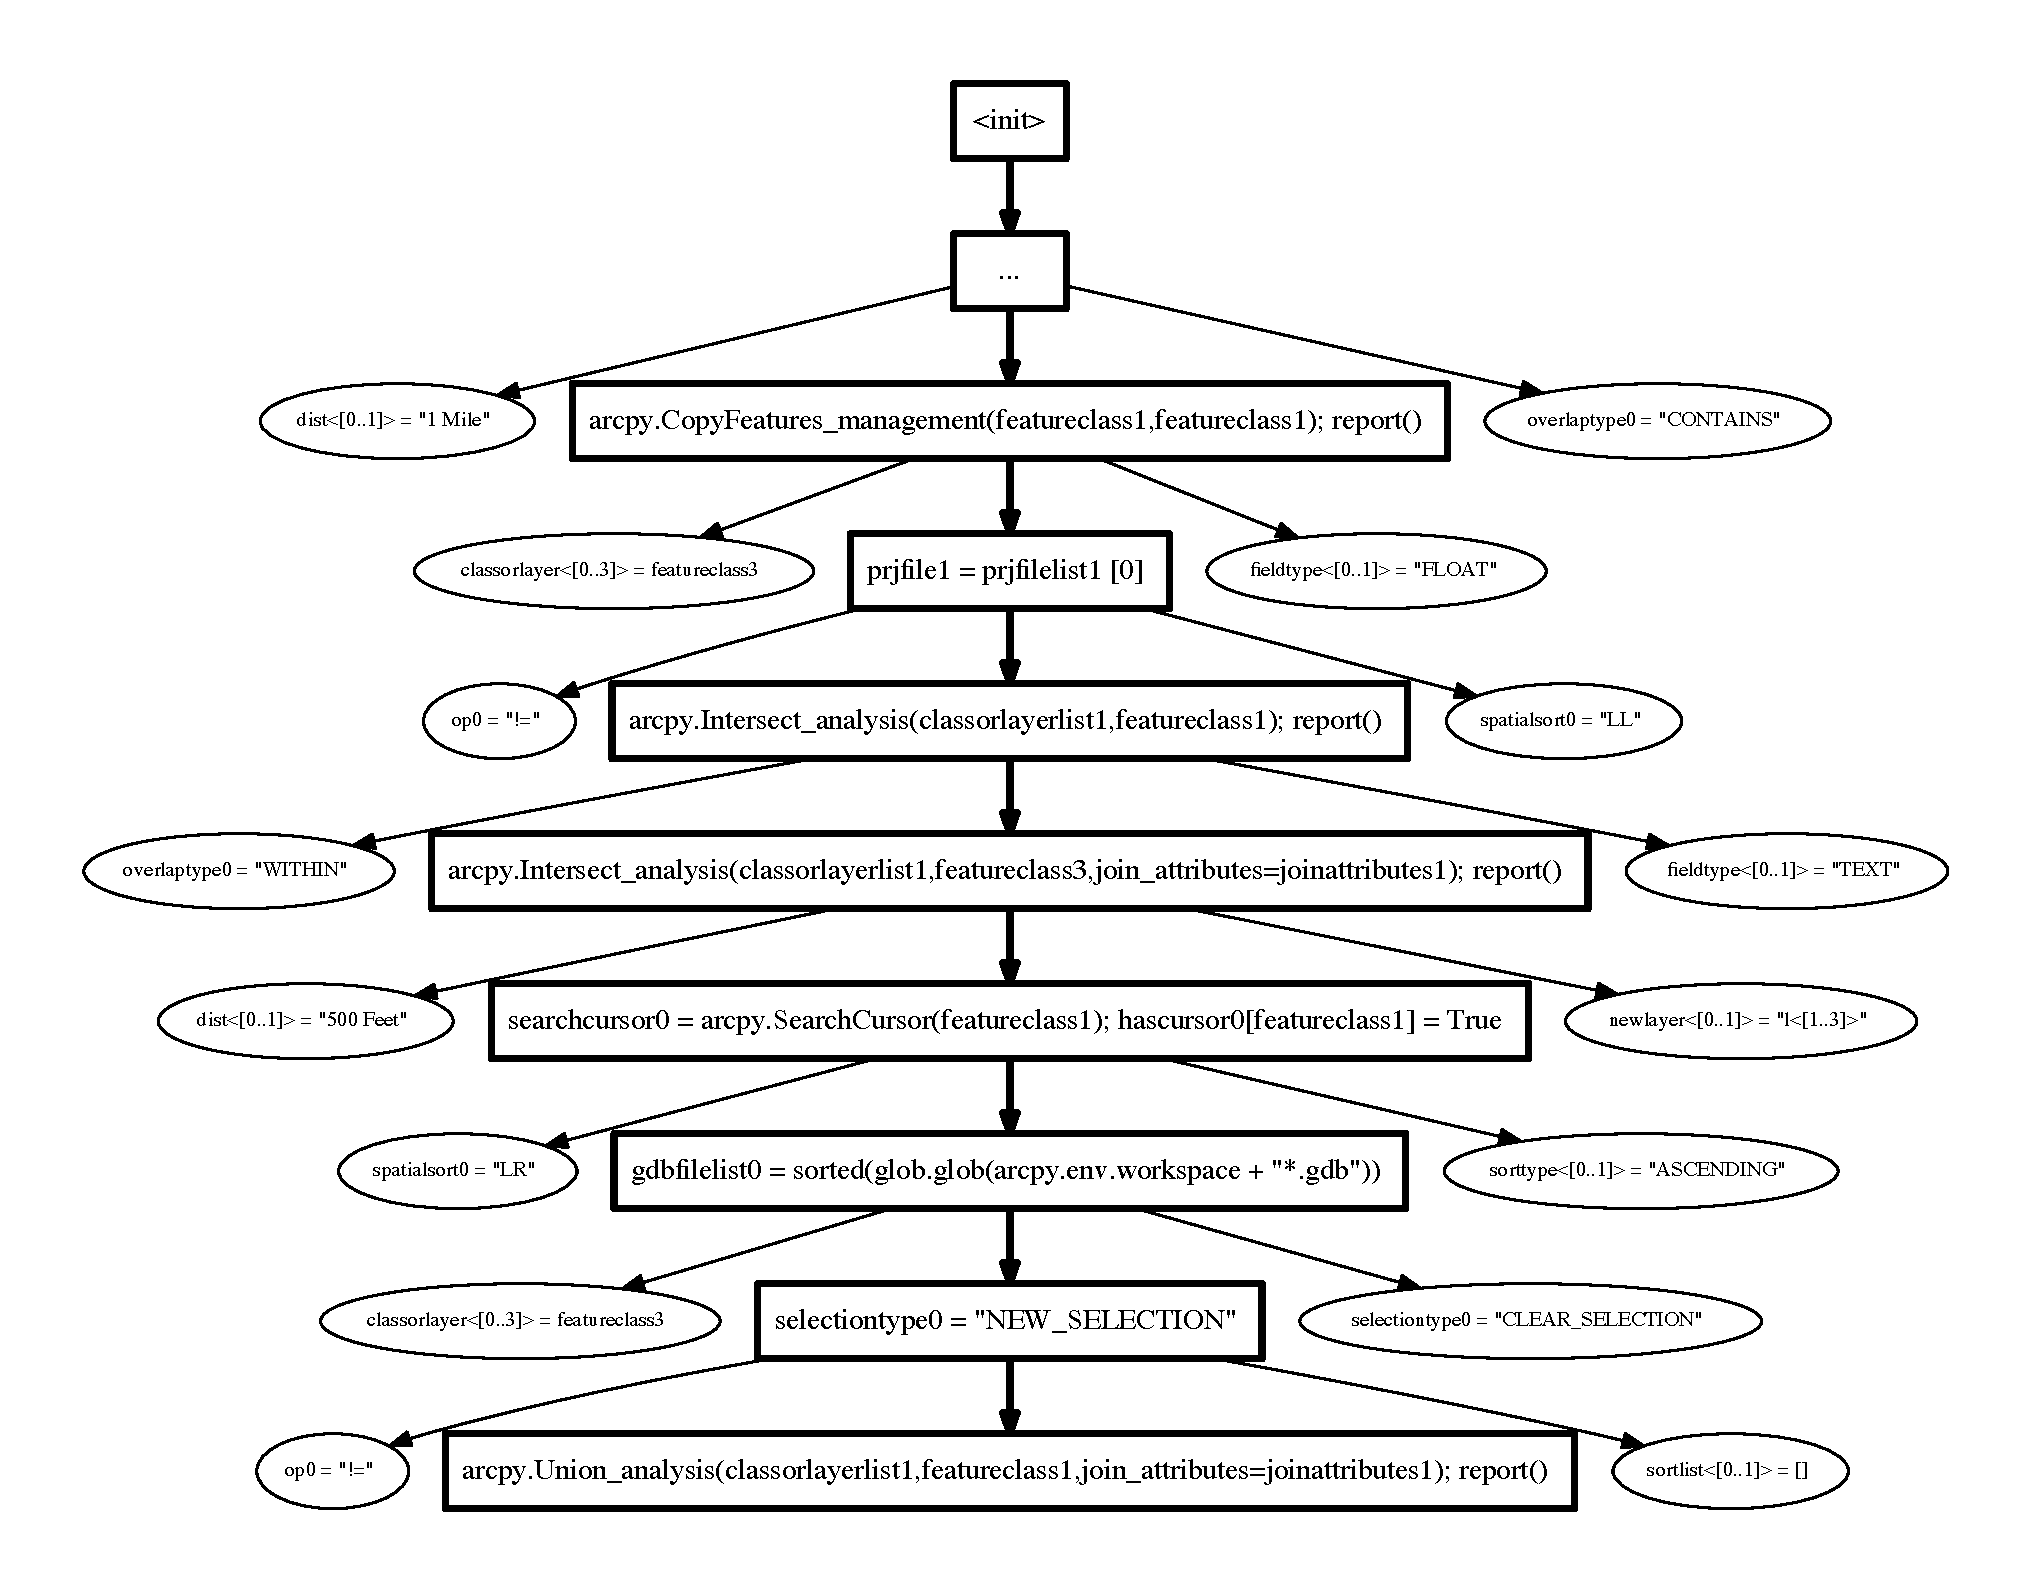
\includegraphics[width=\columnwidth]{shortgraph}
\caption{Start depth 20, depth 8, width 3 trace visualization for ArcPy testing.}
\label{fig:actions}
\end{figure}

Understanding the structure of the action graph produced by even a relatively simple TSTL harness can be difficult.  The structure is often infinite, and even in cases where there is a finite state space (perhaps introduced by abstraction) the graph is usually far too large for a convenient display.  However, we have found that a visual representation of typical trajectories through the system can be very helpful for understanding a complex test system.  The {\tt makegraph} utility takes as input a number of traces to produce, a starting depth, additional depth, and a test width.  It then produces in pdf form a number of graphs for traces like the one shown in Figure \ref{fig:actions}.  These trace graphs show, in bold, the actual action sequence chosen by a pure random tester, starting after a number of actions not shown (represented by the ``...'' node) and continuing up to the depth limit.  In addition to the actions taken, the graph also shows a random subset of additional enabled actions, with each step showing a number of actions equal to the width.  Because many actions are extremely similar, the graphing utility also summarizes actions that are the same, except for pool choice or integer constant, using the {\tt <[i..j]>} notation of TSTL.

\subsection{Building Your Own Testing Tools in TSTL}
\label{sec:build}

Describing the full interface provided by TSTL for use in testing tools is beyond the scope of this paper.  However, examining the source code of the included testers can provide a good starting point.  Implementing new test case manipulations usually involves understanding TSTL internal structures and how tests are stored.  Implementing novel test generation algorithms can often rely on just a handful of methods, shown in Figure \ref{methods} (TSTL provides nearly 100 methods for generating and manipulating tests, but this minimal set can implement many test generation algorithms).

\begin{figure}
{\scriptsize
\begin{itemize}
\item {\bf restart():}  resets the system state and aborts the current test. 
\item {\bf test():} returns the current test.
\item {\bf replay(test):} replays a test, and returns a Boolean indicating success or failure of the test.
\item {\bf enabled():} returns a list of all currently enabled actions.
\item {\bf randomEnabled(random):}  given a Python random number generator object, returns a random enabled action, efficiently (avoiding unnecessary guard evaluations).
\item {\bf safely(action):} performs action (usually changing SUT state)  and returns a Boolean indicating whether the action performed raised any uncaught exceptions. 
\item {\bf check():} returns a Boolean indicating whether any properties fail for the current state.
\item {\bf error():} returns either {\tt None} (no error for the last action or {\tt check}), or a Python object representing an uncaught exception or failed property's backtrace.
\item {\bf state():} returns the current SUT state, as a set of values for all pools; for systems where state cannot be restored by pool values, or {\tt deepcopy} does not work, returns the current test.
\item {\bf backtrack(state):} takes a state or test produced by {\tt state} and restores the system to it.
\item {\bf reduce(test,predicate):} takes a test and a predicate (function from test -> boolean), and returns a (possibly smaller) test also satisfying the predicate).
\item {\bf allBranches():} returns the set of branches covered during all testing.
\item {\bf newBranches():} returns the set of branches covered during the last action executed that had not previously been covered.
\item {\bf currBranches():} returns the set of branches covered during the current test.
\item {\bf saveTest(test, filename):} saves a test in a file.
\item {\bf loadTest(filename):} loads a test from a file (and returns that test as the function's return value).
\end{itemize} 
}
\caption{Some core methods for testing an SUT.}
\label{methods}
\end{figure}

For example, a researcher aware of the literature showing that for many systems it is difficult to outperform random testing, due to its very low overhead \cite{ISSRE12,ISSTA12}, may consider simple modifications of random testing that do not greatly increase overhead.  One such example, with implementation, is shown in the original TSTL paper \cite{NFM15}.  We present another here.  Since the focus of this paper is on showing how to use TSTL, not novel test generation methods, we leave a complete development and statistically valid evaluation of our proposed approach to future work, but discuss briefly how to go about prototyping and evaluation using TSTL.

The idea is to perform random testing, but keep the final state of tests with unusually high coverage as potential starting points for future tests, potentially extending them far beyond the normal test length limit.  The approach is parameterized by {\tt MEMORY}, the number of ``good'' tests to store, by {\tt PEXTEND}, the probability of choosing to extend a ``good'' test rather than start a new test, by the {\tt TEST\_LENGTH} and by a {\tt TIMEOUT} parameter.  Leaving out imports and other boilerplate, the entire implementation is shown in Figure \ref{fig:keepgood}.

\begin{figure}
{\scriptsize
\begin{code}
goodTests = []
startTime = time.time()
while (time.time() - startTime <= TIMEOUT):
   if (len(goodTests) > 0) and (rgen.random() < PEXTEND):
     sut.backtrack(rgen.choice(goodTests)[1])
   else:
     sut.restart()
   for s in xrange(0,TEST\_LENGTH): 
      action = sut.randomEnabled(rgen)
      r = sut.safely(action)
      if len(sut.newBranches()) > 0:
         print time.time(),len(sut.allBranches()),'NEW BRANCHES:', sut.newBranches()
   if MEMORY > 0:
      goodTests.append((sut.currBranches(), sut.state()))
      goodTests = sorted(goodTests, reverse=True)[:MEMORY]
\end{code}
}
\caption{Implementing a very simple novel testing algorithm.}
\label{fig:keepgood}
\end{figure}

\begin{figure}
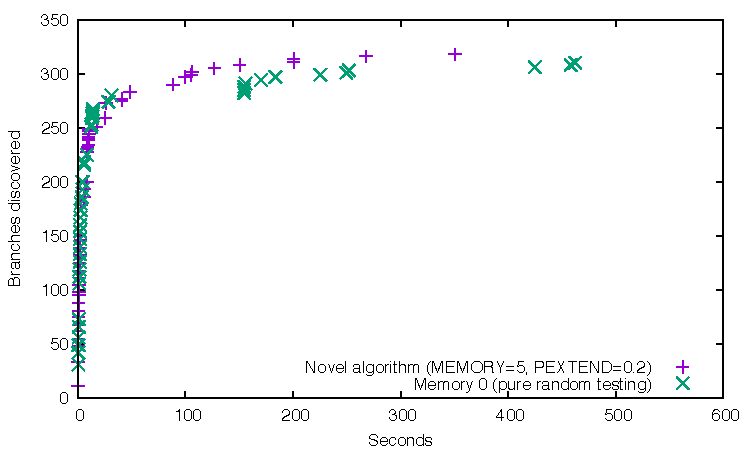
\includegraphics[width=\columnwidth]{memory}
\caption{Comparing branch coverage for 10 minute runs of two test generation methods.}
\label{fig:compare}
\end{figure}

The implementation is trivial, relying only on the TSTL API and some very simple Python tools (sorting with automatic lexical ordering, time library, etc.).  We omit handling of failed tests, assuming the goal of this algorithm is simply to improve code coverage in fault-free systems for experimental evaluation.  This simple tool can be applied to any TSTL harness and will produce output showing when, in time, new branches were covered by the system.  This data can be used to produce Average-Percent-Branches-Detected (APBD) values and discovery curves \cite{issta14,Rothermel1999,rothermel01oct}. Comparison with simple random testing is easy, since setting {\tt MEMORY} to 0 gives pure memoryless random testing (alternatively, to avoid the overhead of the comparisons with 0, a dedicated version for random testing can be written).  A major threat to validity in many comparisons of testing or explicit-state model checking algorithms is that different underlying infrastructure for different algorithms may end up outweighing even moderately sized effects due to the underlying algorithms.  With TSTL, fair comparisons are much easier, since the TSTL interface does most of the computational work that is common to multiple algorithms, with the same overhead.  Evaluating an algorithm can be as simple as finding a large number of suitable programs without failures (or where failures don't make coverage values invalid) and performing enough trials to establish statistical validity for comparisons with APBD values for known algorithms.  Evaluation in terms of discovered faults or time-until-discovery of a fault is nearly as simple.  This algorithm is of some interest, in that while it requires backtracking, the frequency of backtracking is low enough to be potentially applicable even to systems like ArcPy where backtracking is only possible via expensive test replay.  While a mature version of this method would require many SUTs and experiments, as well as investigation of suitable values for {\tt MEMORY} and {\tt PEXTEND}, Figure \ref{fig:compare} shows that average branch discovery curves for ArcPy can sometimes be improved, even using the  arbitrarily chosen parameters of a size 5 memory and a 20\% probability of using a ``good'' test as a starting point.  The simplicity of the Python implementation makes performing automatic experiments with different parameters and test lengths trivial.  Experiments can also take advantage of Python libraries for automatic statistical analysis and plotting of results.


\section{TSTL as a Testing Library Generator}
\label{sec:langext}

While TSTL is easily used as ``just another tool'' that allows testing of an SUT, plus a ``construction kit'' to build your own testing tools, TSTL can also be understood as a generator of libraries.  ArcPy is a site package that makes it easy to perform GIS tasks using Python.  NumPy \cite{NumPy} and SciPy \cite{SciPy} are libraries that make performing scientific computing tasks easy with Python.  QIIME \cite{QIIME}, Biopython \cite{biopython}, and scikit-bio \cite{scikitbio} are libraries that make performing bioinformatics tasks easy using Python.  Such libraries can be of great importance in their subject domains:  ArcPy is extremely widely used, and the subject of university courses in many GIS programs, and the Nature Methods paper introducing QIIME has been cited more than 5,000 times to date, according to Google Scholar.  TSTL, also, can be seen as a tool that generates a library making it easy to perform testing tasks \emph{for a specific SUT}, using Python. 

ArcPy, NumPy, QIIME and the other libraries can be seen as introducing the entities essential to their respective tasks as first-class, easily manipulable objects in the Python language.  TSTL makes tests (for a specific SUT, but using a common interface across all SUTs) first-class, easily manipulable objects.  TSTL does for tests, SUT state, and code coverage what ArcPy does for feature classes, spatial references, and other GIS concepts, what NumPy does for efficiently represented arrays and matrices, and what QIIME does for protein sequences.

The key to understanding TSTL as a library generator is the idea of a test.  A TSTL test is a list of actions\footnote{We expect this type to be the same for any TSTL version for any language:  a list is the simplest way to express pure sequence, which is the essence of a test.}.  The individuals of the action type are dependent on the SUT.  TSTL allows the user to generate, manipulate, and inspect tests in the same way NumPy lets a user explore the behavior of arrays.  This means that TSTL can also be used interactively, as the following example (using some TSTL-supplied methods not shown in Table \ref{methods}) shows:

{\scriptsize
\begin{code}
 >>> import sut, random
 >>> sut = sut.sut()
 >>> r = random.Random()
 >>> (t1, ok) = sut.makeTest(100,r)
 >>> print ok
 True
 >>> sut.prettyPrintTest(t1)
 fieldname1 = "newf1"                                                      \# STEP 0
 polytable0 = arcpy.env.workspace + "\\polyneig.dbf"                        \# STEP 1
...
 arcpy.Erase\_analysis(classorlayer0,classorlayer1,featureclass0); report() \# STEP 98
 arcpy.Buffer\_analysis(classorlayer3,featureclass0,dist1); report()        \# STEP 99
\end{code}
}

Here, a user generates a length 100 test for ArcPy, and then prints it.  The user can also modify the test slightly, using standard Python list modification, generate another test, produce a third test that is the \emph{composition} of the first two tests, and reduce that third test to remove any redundant (with respect to code coverage) steps in it.

{\scriptsize
\begin{code}
 >>> t1[1] = sut.playable(t1[1][0].replace("newf1","newf2"))
 >>> (t2,ok) = sut.makeTest(100,r)
 >>> print ok
 True
 >>> t3 = t1 + t2
 >>> sut.replay(t3)
 >>> bc = sut.currBranches()
 >>> t4 = sut.reduce(t3, sut.coversBranches(bc))
 >>> len(t4)
 78
...
\end{code}
}

The user is causing ArcGIS to perform GIS operations, but without specifying those operations; the GIS tasks are conceptually reduced to the actions of an arbitrary SUT, but the printed test makes it clear what is going on at the SUT level.  While this example shows the {\tt makeTest} interface being used with the default generator (pure random testing), a user can supply a more complex generator as a function.  For example, to implement testing such that if the last action resulted in any new coverage, it is repeated, a user could first
define a generator function (assume that {\tt r} is a random number generator defined globally, as above):

{\scriptsize
\begin{code}
def repeatGen(lastAction,sut):
   if (lastAction != None) and (len(sut.newBranches()) > 0) and (lastAction[1]()):
      return (lastAction, lastAction)
   newAction = sut.randomEnabled(r)
   return (newAction, newAction)
\end{code}
}
and then generate a length 100 test using this strategy easily:
{\scriptsize
\begin{code}
 >>> (t5, ok) = sut.makeTest(100, sgenerator=repeatGen)
\end{code}
}

The function {\tt repeatGen} takes a state (initially {\tt None} to indicate a new test) consisting of a single action --- the last action executed.  It then, if there is a{\tt lastAction}, and the last step of testing increased branch coverage, and the action is still enabled, returns that action as both the next action to perform and the new state of the generator.  Otherwise, it generates a random action, and returns that as the state and the action.

We do not believe such an interactive approach to testing is natural with most other tools that generate either model checking traces or method-call sequence tests.  In fact, the very idea of test case composition as shown in the first interactive code fragment may seem quite strange to users of either model checking or conventional unit tests.  Although TSTL tests are sequences of actions --- essentially small, deterministic programs with no inputs --- they can be interacted with and generated like tests in QuickCheck \cite{ClaessenH00} or Hypothesis \cite{hypothesis}, where tests are usually just function inputs (lists, data structures, etc.). This ease-of-use for exploratory testing is a primary reason TSTL was first implemented for Python, rather than a compiled language such as Java or C (hence the ``Scripting'' part of ``Template Scripting Testing Language'').  A Swift, Ruby, or Scala version would also provide a way to interact with tests in a simple, immediate, and basically ``functional'' way.



\section{Faults Discovered Using TSTL}
\label{sec:bugs}

\subsection{ArcPy Faults}

\begin{figure}
{\scriptsize 
\begin{code}
shapefilelist0 = glob.glob("C:\\Arctmp\\*.shp")                             \textcolor{black!60}{\# STEP 0}
\textcolor{black!60}{\#[}
shapefile0 = shapefilelist0 [0]                                           \textcolor{black!60}{\# STEP 1}
newlayer0 = "l1"                                                          \textcolor{black!60}{\# STEP 2}
\textcolor{black!60}{\#  or newlayer0 = "l2" }
\textcolor{black!60}{\#  or newlayer0 = "l3" }
\textcolor{black!60}{\#  swaps with steps 3 4 5 6 7}
\textcolor{black!60}{\#] (steps in [] can be in any order)}
\textcolor{black!60}{\#[}
featureclass0 = shapefile0                                                \textcolor{black!60}{\# STEP 3}
\textcolor{black!60}{\#  swaps with step 2}
fieldname0 = "newf1"                                                      \textcolor{black!60}{\# STEP 4}
\textcolor{black!60}{\#  or fieldname0 = "newf2" }
\textcolor{black!60}{\#  or fieldname0 = "newf3" }
\textcolor{black!60}{\#  swaps with steps 2 8}
selectiontype0 = "SWITCH\_SELECTION"                                       \textcolor{black!60}{\# STEP 5}
\textcolor{black!60}{\#  or selectiontype0 = "NEW\_SELECTION" }
\textcolor{black!60}{\#  or selectiontype0 = "ADD\_TO\_SELECTION" }
\textcolor{black!60}{\#  or selectiontype0 = "REMOVE\_FROM\_SELECTION"}
\textcolor{black!60}{\#  or selectiontype0 = "SUBSET\_SELECTION"}
\textcolor{black!60}{\#  or selectiontype0 = "CLEAR\_SELECTION"   }
\textcolor{black!60}{\#  swaps with steps 2 8}
op0 = ">"                                                                 \textcolor{black!60}{\# STEP 6}
\textcolor{black!60}{\#  or op0 = "<" }
\textcolor{black!60}{\#  swaps with steps 2 8}
val0 = "100"                                                              \textcolor{black!60}{\# STEP 7}
\textcolor{black!60}{\#  or val0 = "1000" }
\textcolor{black!60}{\#  swaps with steps 2 8}
\textcolor{black!60}{\#] (steps in [] can be in any order)}
arcpy.MakeFeatureLayer\_management(featureclass0, newlayer0)               \textcolor{black!60}{\# STEP 8}
\textcolor{black!60}{\#  swaps with steps 4 5 6 7}
arcpy.SelectLayerByAttribute\_management(newlayer0,selectiontype0,
   ' "'+fieldname0+'" '+op0+val0)                                         \textcolor{black!60}{\# STEP 9}
arcpy.Delete\_management(featureclass0)                                    \textcolor{black!60}{\# STEP 10}
arcpy.SelectLayerByAttribute\_management(newlayer0,selectiontype0,
   ' "'+ fieldname0+'" '+op0+val0)                                        \textcolor{black!60}{\# STEP 11}
\end{code}
}
\caption{Deleting a feature class does not invalidate or delete layers that depend on it.}
\label{fault1}
\end{figure}

In the process of testing ArcPy with TSTL, we discovered at least five
distinct faults
(thus far) that can cause an ArcPy script to crash.  While we have (as
discussed in Section \ref{sec:lang}) some properties that check for
data corruption and determinism of GIS analysis, we are not focusing
on these until we have a reliable way to avoid system crashes.   In
order to give an idea of what TSTL test cases look like, we discuss
briefly one of these ArcPy crashes.

ArcPy crashes when the feature class from which a layer is produced is
deleted, and the layer is used in a {\tt SelectLayer} call (this
version shows an attribute-based selection, but location selection
will cause the same problem): (Figure \ref{fault1}).  The underlying issue seems to be that
while operations on a deleted feature class properly notify a user the
feature class does not exist, ArcPy or ArcGIS does not track that
layers produced from a feature class should also be deleted/invalidated
when the feature class is deleted.  Layers are not copies
of a feature class, but essentially new \emph{views} of a feature class.
This means that when the underlying feature class is modified or
deleted, the view needs to be updated to reflect that change, and this
is not correctly implemented.  Figure \ref{fault1} shows part of an
annotated, reduced, normalized, and generalized test stand-alone test
case (with the boilerplate, function definitions, and imports
removed) for this fault.  The final line of code crashes ArcPy and the
Python interpreter.  Comments indicate alternative similar tests that
also fail.  In this case, TSTL's additional reduction steps (based on
term rewriting in the action language) remove almost half the steps in
the original, delta-debugged test case.

Other faults (or documentation lapses) in ArcPy we have discovered include crashes when computing
statistics over database fields of a layer using a deleted field and
crashes due to seemingly reasonable modifications of feature classes
while a database cursor is active.  In order to deal with the latter,
which seems more in the line of an undocumented behavioral restriction
than a ``bug,'' we now drastically limit database modification when a
cursor is active.  We have reported these problems to Esri, but have
not received a response.  The problems discovered may be previously
known to Esri, but are not generally known to the ArcPy user
community, and those that could be considered API limitations (that
cause unexplained crashes when violated) are not documented.

\subsection{Faults in Other Systems}

TSTL  is only slightly less than two years old, and a stable, mature,
non-prototype version has only existed for about a year.   However,
TSTL has already been used to find important bugs in real systems.

Using TSTL's support for differential testing, we were able to 
quickly find 
and report issues with the widely-used {\tt gmpy2} interface to the GMP (GNU 
Multiple Precision \cite{gmp} arithmetic library), as well as 
(surprisingly) in the core CPython bignum implementation
\cite{gmpy2bugs,cpythonbug}. 


TSTL was also able to discover at least 15
previously undiscovered faults in the widely used SymPy library for
symbolic mathematics in Python \cite{sympy}.  We have reported these
faults, and hope to collaborate with the SymPy team to provide
assistance in localizing and fixing them using TSTL.  The SymPy
effort was able to move from
decision-to-test to first discovered fault in the course of a single
day, due to the much higher ease-of-use for the post-ArcPy version of
TSTL used.  For a straightforward testing task like SymPy, building a
TSTL harness is now quite simple, largely a matter of thinking about
what the user wishes to test.

Students using TSTL in graduate classes on software testing have
already, with minimal assistance, discovered faults in some real-world
systems.  Not all of these are confirmed and reported yet.  TSTL
testing revealed a fault in either the widely-used {\tt PyOpenCL}
library \cite{PyOpenCL}, the even more widely-used {\tt OpenCL}
infrastructure \cite{OpenCL}, or (possibly) the NVIDIA hardware being
used.  We are still investigating this problem, but it appears to be a
genuine fault, though debugging and assigning blame is complex due to
the layers of software and hardware involved.  Second, TSTL testing
found cases where distance metrics that were supposed to be symmetric
in the popular fuzzy-string-matching library FuzzyWuzzy
\cite{FuzzyWuzzy} were asymmetric, if the default Python string match
library was used instead of a Levenshtein-distance library.  Third,
TSTL testing revealed numerous problems with the {\tt astropy.table}
module of the AstroPy library \cite{AstroPy}, used by many
professional astronomers and astrophysicists.  TSTL has also been used
to discover faults in the TSTL API itself.  The github repository for
the graduate class in question
(\url{https://github.com/agroce/cs562w16}) contains the TSTL code for
testing these systems (and many other student projects).


\section{Related Work}

Chen et al. introduced the idea of slippage in the course of
describing efforts to automatically detect different faults in a large
set of failing test cases \cite{PLDI13}.  Hughes et
al. \cite{FindMoreBugs} proposed a modification of QuickCheck
to avoid re-producing known bugs that (in theory)
could mitigate the problem of slippage, but is not directly comparable
to our approach.  The approach of Hughes et al. requires
interpretation of test components (e.g. method calls), and analysis of
patterns, while our approaches are purely algorithmic, with no
additional requirements beyond those of delta debugging itself
\cite{DD}.  It is not clear how best to apply such an approach
 to cases such as {\tt jsfunfuzz} where each component is not a
method call but essentially an arbitrary string, without significant
user effort to define abstractions of components.

There are also approaches that sidestep slippage by initially
producing short test sequences (e.g. recent work by Mao et
al. \cite{Mao}).  However, for many generation algorithms
longer sequences are essential for good fault detection \cite{ASE08,LongBetter}.

\section{Conclusions}
\label{conclusion}

This paper reports on an end-user-driven automated testing effort for a Python
library used to automate Geographic Information System analysis and
data management.  The test system is based on the TSTL
\cite{NFM15,ISSTA15,tstl} domain-specific language for testing, which
enables a declarative style of test harness development, where the
focus is on defining the actions in valid tests, not determining
exactly how tests are generated.

The complexity, size, and some unusual features of
the SUT have driven some engineering decisions, enhancements to the
TSTL language, and new testing utilities.  This paper focuses on
presenting the experience of testing a large complex system, and (we
hope) demonstrates that a domain expert whose programming experience
consists almost entirely of using the Software Under Test can make use
of modern automated test generation methods to find faults in complex software systems.

\bibliographystyle{spmpsci}      % mathematics and physical sciences
%\bibliographystyle{spphys}       % APS-like style for physics
\bibliography{bibliography}   % name your BibTeX data base



\end{document}
% end of file template.tex

